% ================================================================
% The Retrieve and Connect version of latex/starters/targeted/KS4/geometry/trigBearingStarter02.tex
%
% This is the same deck as the one above, made by renaming the titles in it.
% Every slide that was a numbered starter is now titled
% "Retrieve and Connect", and the word is renamed wherever else a title
% used it. Nothing outside a title has been changed.
%
%   made from           latex/starters/targeted/KS4/geometry/trigBearingStarter02.tex
%   retitling rules     version 1
%
% Please don't edit this file. It is written again from the one it was
% made from whenever that changes, so an edit here would be lost - edit
% that file instead and this one follows.
% ================================================================
\documentclass[aspectratio=169,11pt]{beamer}

% ------------------ Theme & basic tweaks ------------------
\usetheme{default}
\usecolortheme{dove} % calm grayscale colours
\setbeamertemplate{navigation symbols}{} % hide nav icons
\setbeamertemplate{footline}[frame number] % show slide numbers

% ------------------ Fonts & symbols ------------------
\usepackage[T1]{fontenc}
\usepackage[utf8]{inputenc}
\usepackage{lmodern} % clean sans font
\usepackage{amsmath, amssymb}
\usepackage{siunitx} % optional: for \ang{53} etc.

% ------------------ TikZ ------------------
\usepackage{tikz}
\usetikzlibrary{arrows.meta, calc, angles, quotes, decorations.markings, positioning}
\usetikzlibrary{angles, quotes}

% ================================================================
% Answer-overlay helpers
% ================================================================
\newcommand{\ablank}[1]{%
  \alt<2>{\textcolor{red}{#1}}{\underline{\phantom{#1}}}%
}
\newcommand{\ashow}[1]{\uncover<2->{\textcolor{red}{\small #1}}}
\newcommand{\ashowq}[1]{\alt<2->{\textcolor{red}{\small #1}}{?}}

% Answers drawn straight on to a TikZ diagram, revealed on overlay 2 like \ashow.
% Space is reserved on overlay 1, so the diagram does not move between slides.
\usetikzlibrary{overlay-beamer-styles}
\tikzset{
  ans/.style     = {red, thick, visible on=<2->},
  ansfill/.style = {red!15, visible on=<2->},
  anslab/.style  = {red, font=\tiny, visible on=<2->},
}

% ------------------ Title (optional) ------------------
\title{Year 10 Retrieve and Connect}
\subtitle{Right-angled Trig, Bearings, and Directions}
\author{Matthew Holmes}
\date{} % leave empty for no date

\begin{document}


\begin{frame}{Retrieve and Connect Questions}

\begin{columns}[t]
% ---------------- LEFT COLUMN ----------------
\begin{column}{0.48\textwidth}

% -------- Question 1: Trig - Find the side --------
\textbf{1.}

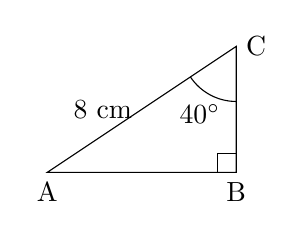
\begin{tikzpicture}[scale=0.8]
% Triangle coordinates
\coordinate (A) at (0,0);
\coordinate (B) at (3,0);
\coordinate (C) at (3,2);

% Draw triangle
\draw (A) -- (B) -- (C) -- cycle;

% Right angle at B
\draw (3,0) rectangle +(-0.3,0.3);

% Labels for vertices
\node[below] at (A) {A};
\node[below] at (B) {B};
\node[right]  at (C) {C};

% Side length AC
\node[left] at ($(A)!0.5!(C)$) {$8\text{ cm}$};

% Angle at C (theta = 40°)
\pic [draw, -, "$40^\circ$", angle eccentricity=1.4, angle radius=0.7cm]
{angle = A--C--B};
\end{tikzpicture}

\vspace{0.3em}
Find the length of BC. \ashow{$8\cos 40^\circ \approx 6.13~\text{cm}$}

% -------- Question 2: Trig - Find the angle --------

\textbf{2.}
\vspace{0.3em}
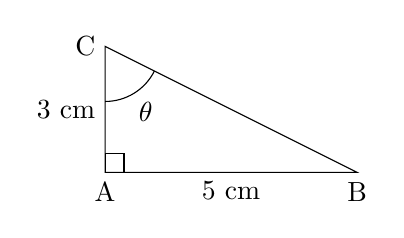
\begin{tikzpicture}[scale=0.8]
% Coordinates
\coordinate (A) at (0,0);
\coordinate (B) at (4,0);
\coordinate (C) at (0,2);

% Triangle
\draw (A) -- (B) -- (C) -- cycle;

% Right angle at A
\draw (A) rectangle +(0.3,0.3);

% Vertex labels
\node[below] at (A) {A};
\node[below] at (B) {B};
\node[left]  at (C) {C};

% Side labels
\node[below] at ($(A)!0.5!(B)$) {$5\text{ cm}$};  % AB
\node[left]  at ($(A)!0.5!(C)$) {$3\text{ cm}$};  % AC

% Angle at C (angle ACB)
\pic [draw, -, "$\theta$", angle eccentricity=1.4, angle radius=0.7cm]
{angle = A--C--B};

\end{tikzpicture}

\vspace{0.3em}
Find $\theta$ \ashow{$\approx 59.0^\circ$}

\end{column}

% ---------------- RIGHT COLUMN ----------------
\begin{column}{0.48\textwidth}

\textbf{3.}

\begin{columns}[T,onlytextwidth]
  \begin{column}{0.55\textwidth}
    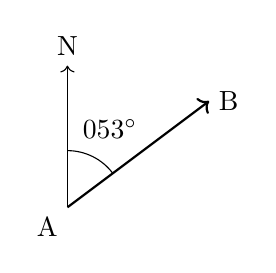
\begin{tikzpicture}[scale=0.9]
      % Points
      \coordinate (A) at (0,0);
      \coordinate (B) at (2,1.5);

      % Bearing line B from A
      \draw[->, thick] (A) -- (B);

      % North at A
      \draw[->] (A) -- +(0,2) node[above] {N};

      % Angle arc at A: 053° clockwise from North
      \draw (0,0) ++(0,0.8) arc[start angle=90, end angle=37, radius=0.8];
      \node at (0.6,1.1) {$053^\circ$};

      % Labels
      \node[below left] at (A) {A};
      \node[right]      at (B) {B};
    \end{tikzpicture}
  \end{column}
  \begin{column}{0.45\textwidth}
    The bearing of \textbf{B from A} is \(\,053^\circ\).\\[0.3em]
    What is the bearing of \textbf{A from B}\,\ashowq{$233^\circ$}
  \end{column}
\end{columns}


% -------- Question 4: Directions at right angles --------
\textbf{4.}

\begin{columns}[T,onlytextwidth]
  \begin{column}{0.55\textwidth}
    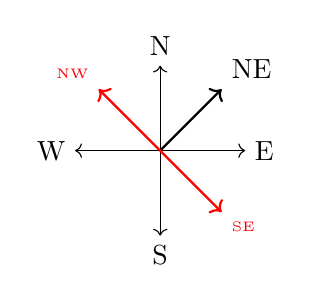
\begin{tikzpicture}[scale=0.6]
      % Compass rose
      \draw[->] (0,0) -- (0,1.8) node[above] {N};
      \draw[->] (0,0) -- (1.8,0) node[right] {E};
      \draw[->] (0,0) -- (0,-1.8) node[below] {S};
      \draw[->] (0,0) -- (-1.8,0) node[left] {W};

      % NE arrow
      \draw[->, thick] (0,0) -- (1.3,1.3) node[above right] {NE};

      % Answer: NW and SE
      \draw[->, ans] (0,0) -- (-1.3,1.3) node[anslab, above left] {NW};
      \draw[->, ans] (0,0) -- (1.3,-1.3) node[anslab, below right] {SE};
    \end{tikzpicture}
  \end{column}
  \begin{column}{0.45\textwidth}
    Which directions are at right angles to \textbf{Northeast}\,?
  \end{column}
\end{columns}

\end{column}
\end{columns}

\end{frame}

\end{document}